Con el desarrollo de la biblioteca ya es posible hacer la implementación de un proyecto el cual ya usa React.
A continuación se ejemplifica el uso de la biblioteca paso a paso.

Existe una herramienta que nos permite crear el esqueleto de una Web basada en React. \cite{CRA}  ( Getting Started | Create React App) esta es desarrollada y mantenida por Facebook, de la cual partiremos para crear una Web en la que probaremos la biblioteca.

Instalaremos la herramienta llamada Create React App con el siguiente comando.
\newline
\begin{figure}[H]
    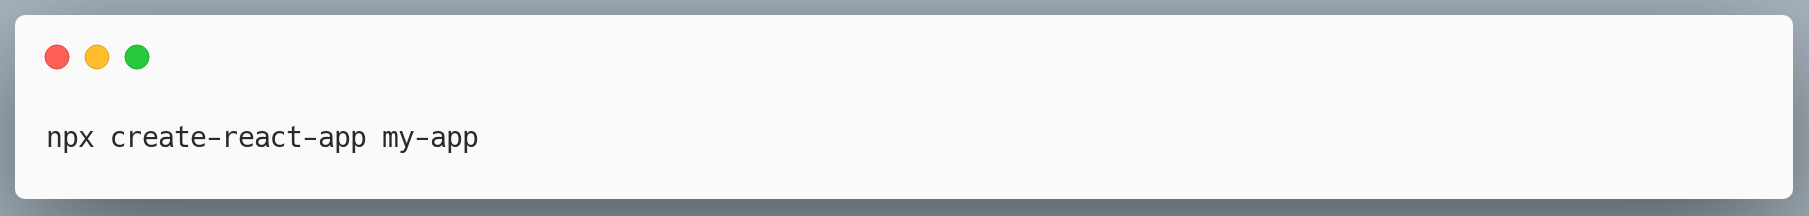
\includegraphics[width=1\textwidth]{./Imagenes/9.1.png}
    \caption[Instalar Create React App]{Instalar Create React App}
    \end{figure}
\newline

Crearemos la Web llamada ejemplo-1 con el siguiente comando.
\newline
\begin{figure}[H]
    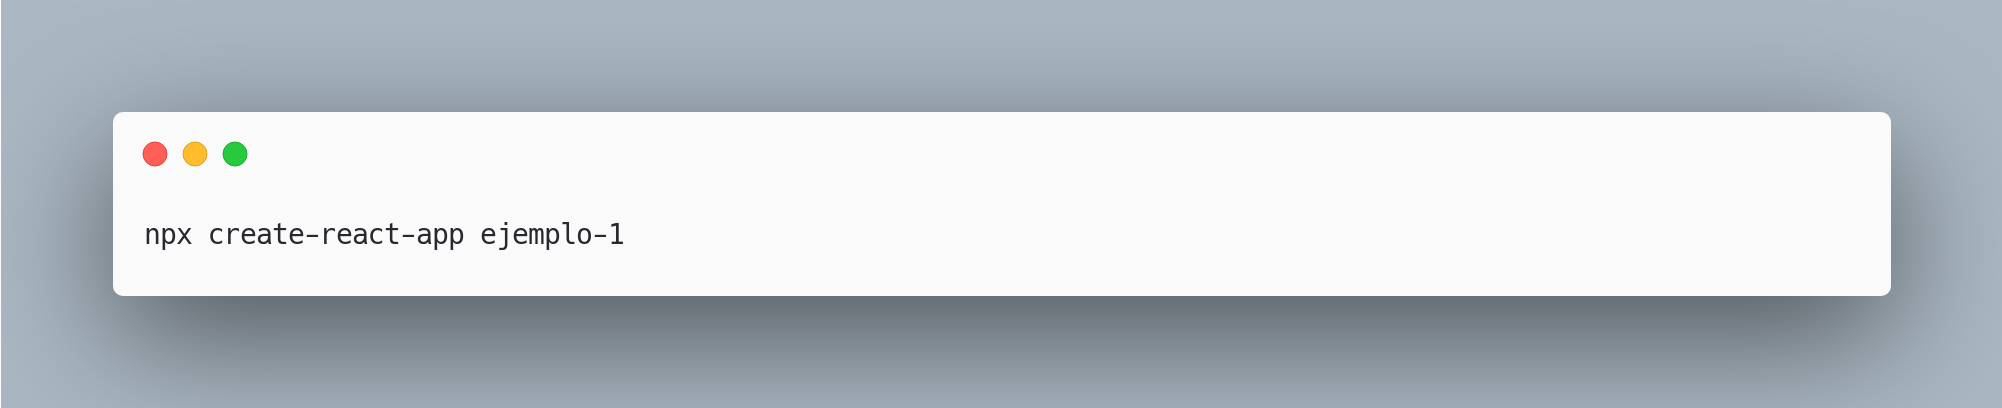
\includegraphics[width=1\textwidth]{./Imagenes/9.2.png}
    \caption[Crear una nueva app]{Crear una nueva app}
    \end{figure}
\newline

El comando nos generará los siguientes directorios.
\newline
\begin{figure}[H]
    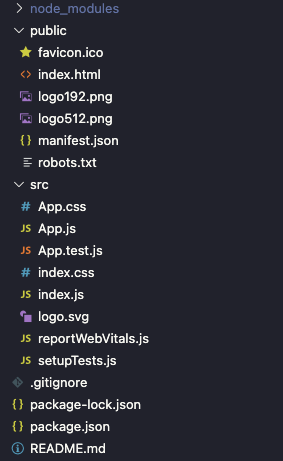
\includegraphics[width=0.5\textwidth]{./Imagenes/9.3.png}
   \centering 
    \caption[Directorios al crear una nueva app]{Directorios al crear una nueva app}
    \end{figure}
\newline

Para poder probar nuestra biblioteca debemos a indicar a la app ejemplo-1 que use la dependencia instalándola con el siguiente comando.\newline
\newline
\begin{figure}[H]
    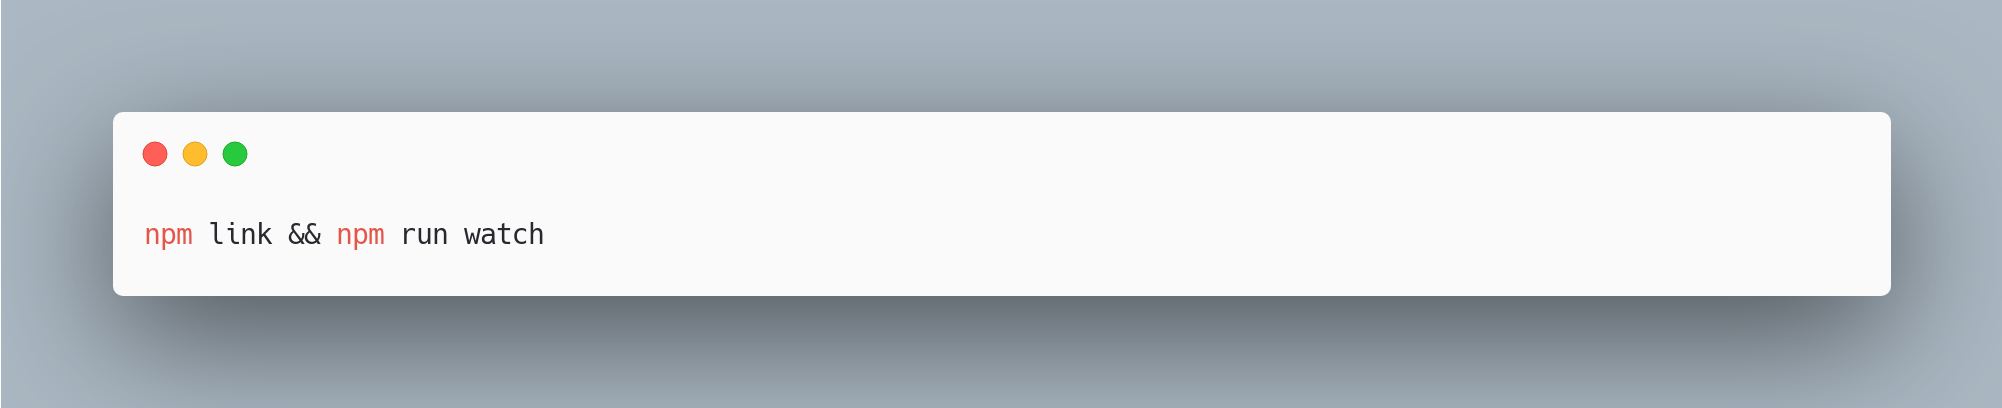
\includegraphics[width=1\textwidth]{./Imagenes/9.4}
   \centering 
    \caption[Instalando nuestra biblioteca]{Instalando nuestra biblioteca}
    \end{figure}
\newline

Ahora basta incluirlo como se agrega cualquier dependencia de node, basta con agregar cualquiera de los elementos aquí desarrollados. 

Crearemos dos ejemplos simples para mostrar el funcionamiento de la biblioteca desde el lado Front-end, cabe aclarar que no se tratará el tema de cómo procesar los datos hacia el Back-end.
El primero consta de un formulario el cual solicita nombre, correo electronico y contraseña, esto con el objetivo de registrar un usuario para que tenga un correo institucional, también se le solicitará si la cuenta estará activa al momento de crearla.

Para esto debemos importar nuestros componentes de la siguiente manera.
\newline
\begin{figure}[H]
    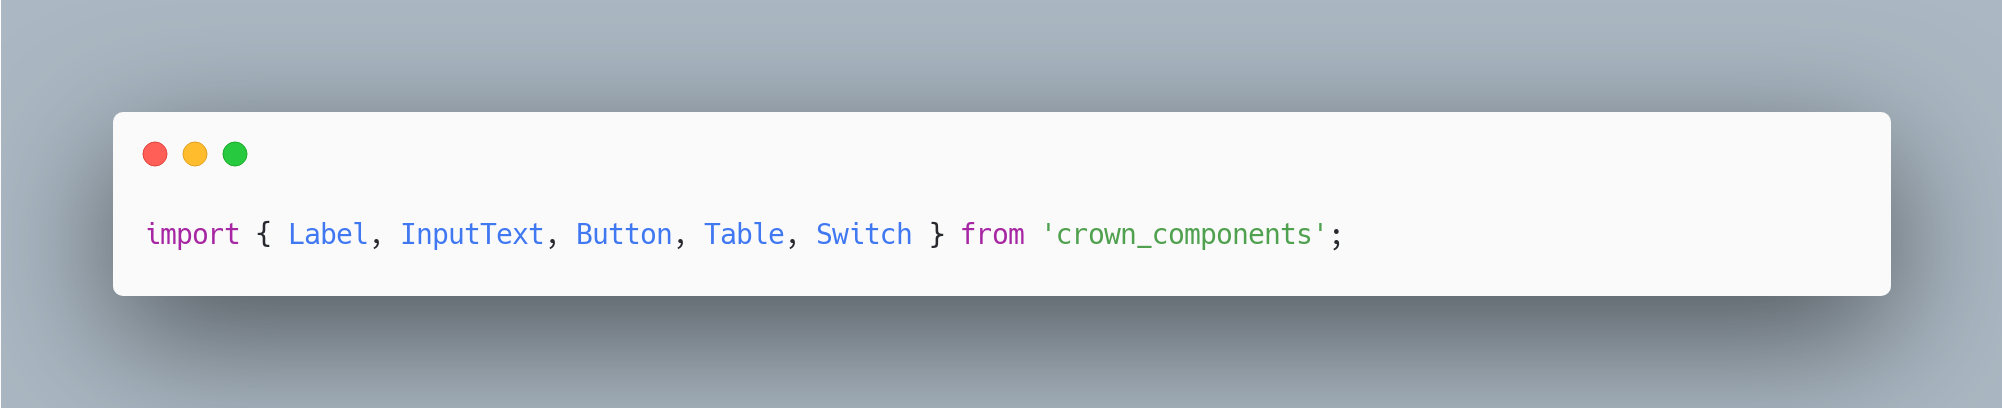
\includegraphics[width=1\textwidth]{./Imagenes/9.6}
   \centering 
    \caption[Implementación la biblioteca]{Implementación la biblioteca}
    \end{figure}
\newline

Después en el estado de React debemos agregar algunos campos para almacenar la información del formulario como se muestra en la siguiente figura.
\newline
\begin{figure}[H]
    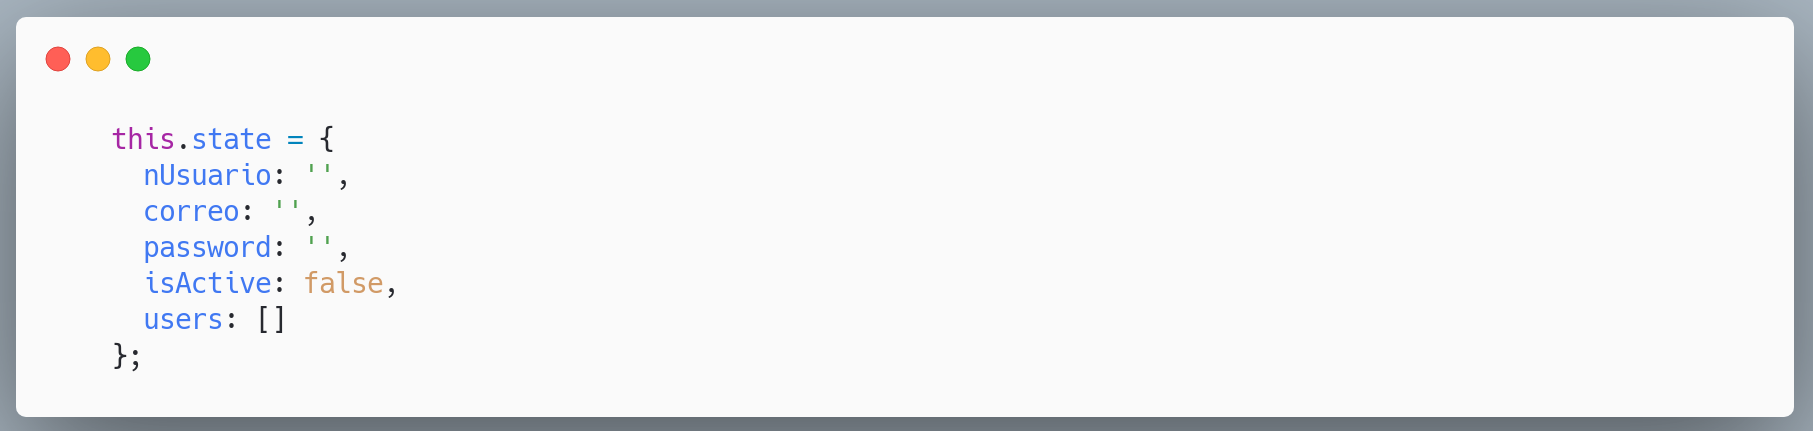
\includegraphics[width=1\textwidth]{./Imagenes/9.7}
   \centering 
    \caption[Agregar campos al estado de React]{Agregar campos al estado de React}
    \end{figure}
\newline
Los datos se usarán para:

  \begin{itemize}
   \item \textbf{ nUsuario:} Nombre de usuario del nuevo registro.
   \item \textbf{ correo:} Correo del usuario.
   \item \textbf{ password:} Contraseña del usuario.
   \item \textbf{ isActive:} Activar la cuenta al crearla.
   \item \textbf{ users:} Usuarios registrados, esto simulando nuestra base de datos.
  \end{itemize}

En la siguiente imagen se muestra el código necesario para desplegar en pantalla el formulario requerido así como una tabla para mostrar los usuarios registrados.

\newline
\begin{figure}[H]
    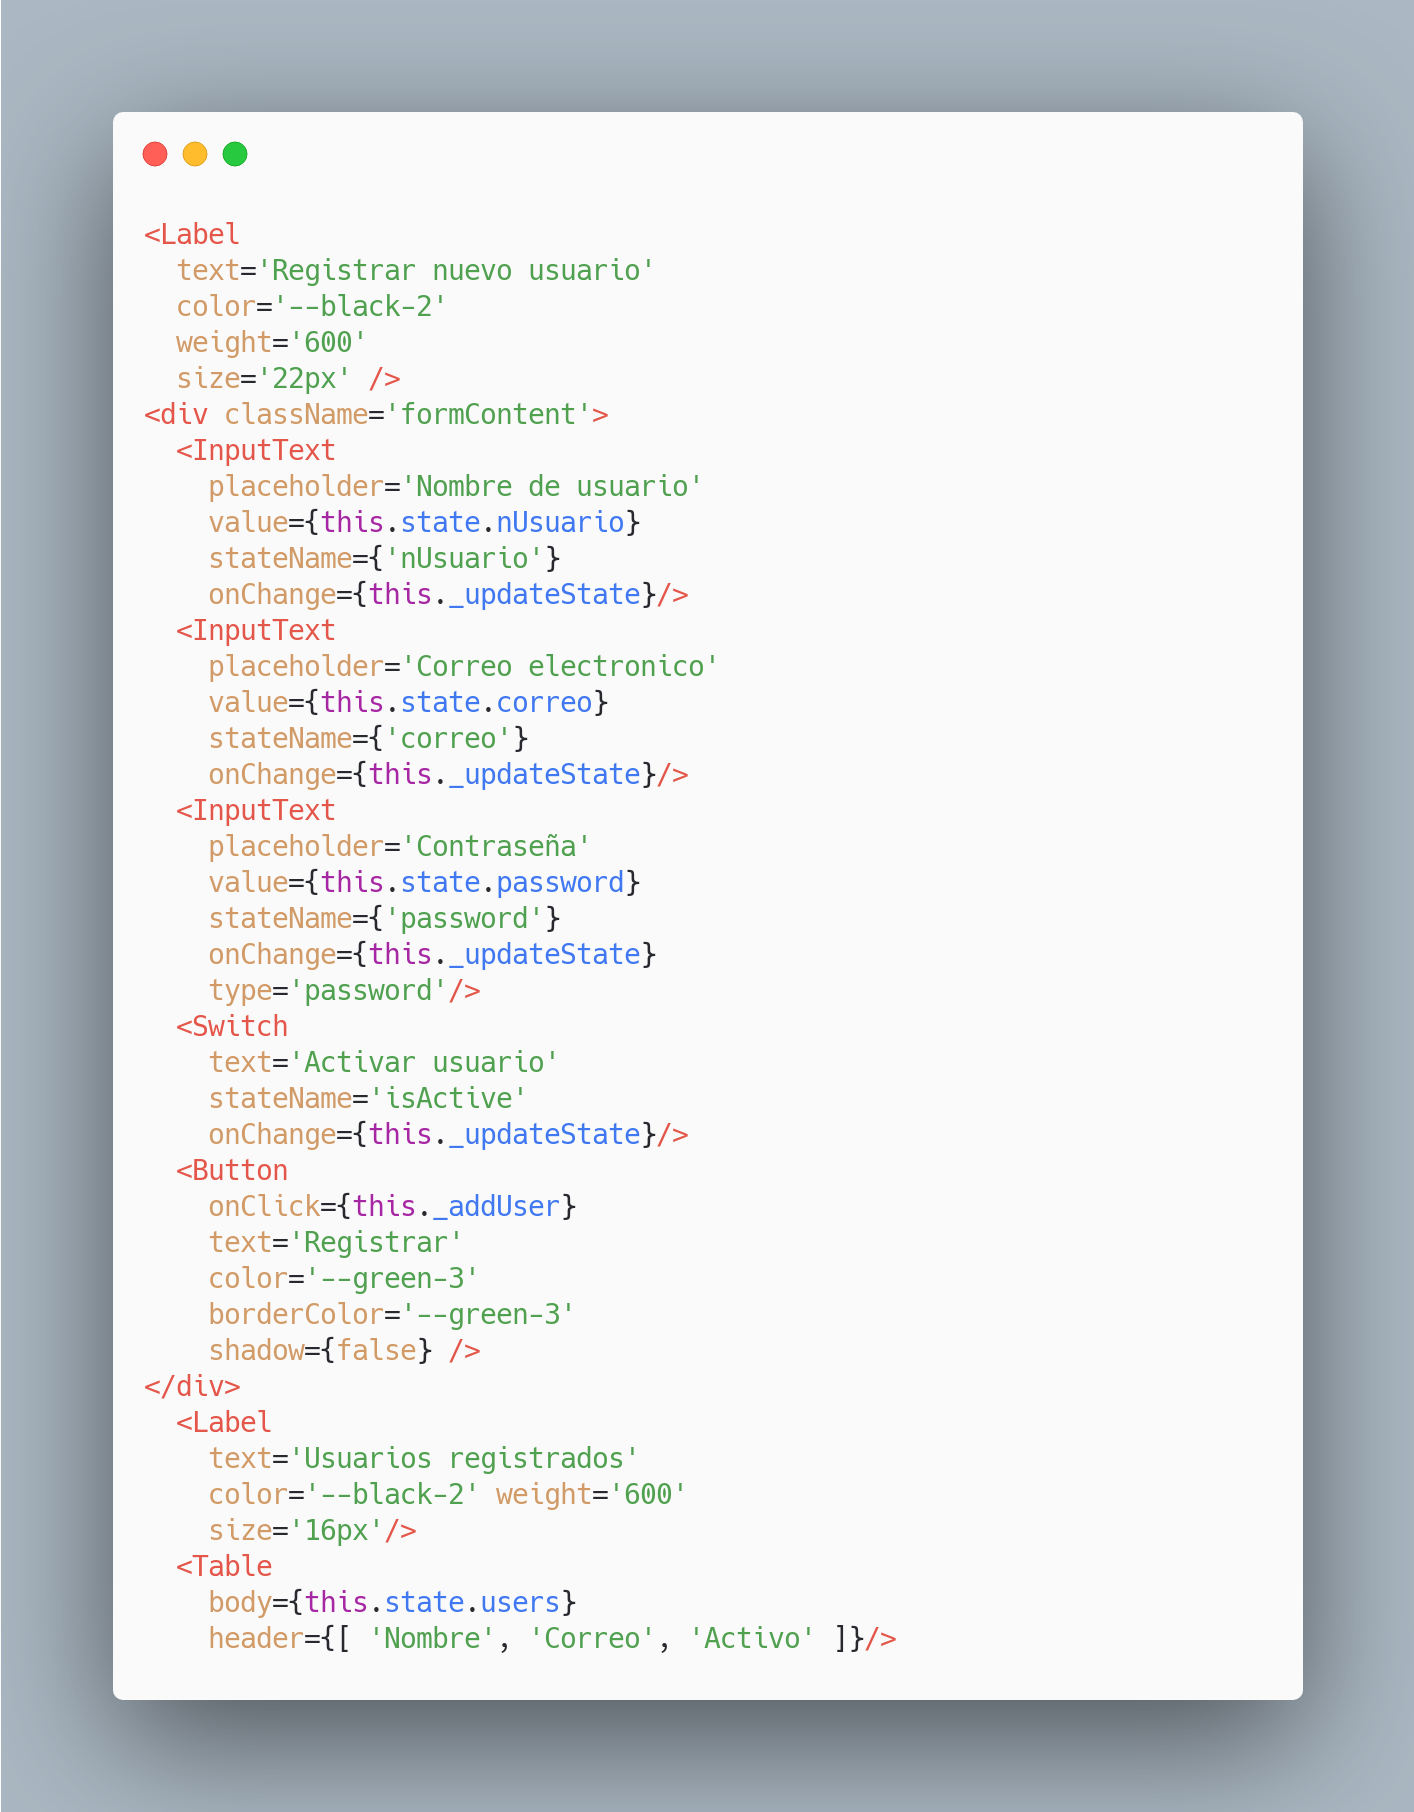
\includegraphics[width=1\textwidth]{./Imagenes/9.8}
   \centering 
    \caption[Código para maquetar]{Código para maquetar}
    \end{figure}
\newline

El código contiene al inicio un componente Label el cual muestra en pantalla un texto dado con las especificaciones de preferencia, se le da un tamaño de letra y color del texto. Después siguen una serie de InputText los cuales son la entrada de datos para el nombre de usuario, correo electronico  y contraseña, Estos tienen parámetros que son importantes de mencionar ya se son indispensables para el correcto funcionamiento como son:
placeholder: Es el texto que se mostrará en el campo de texto antes de que se introduzca un dato, para dar una pista del dato solicitado.
value: Es el estado de React en el que se almacenará cuando ocurra un cambio.
stateName: Es la forma en como es llamado en el estado de React ( Ejemplo. en este caso sería alguna de las llaves que se muestran en la Figura 9.6 ).
onChange: Es la función que se activará cuando algún dato se actualice.

El último parámetro onChange es una función simple como la que se muestra a continuación. 

\newline
\begin{figure}[H]
    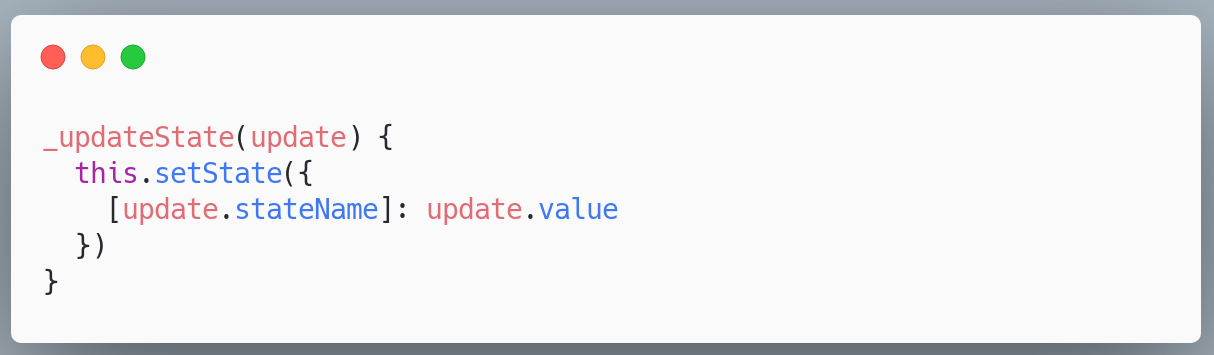
\includegraphics[width=1\textwidth]{./Imagenes/9.9}
   \centering 
    \caption[Función para actualizar el estado de React]{Función para actualizar el estado de React}
    \end{figure}
\newline

Esta función es única para cualquiera de los componentes de la biblioteca, ya que están diseñados para que cuando se actualicen, regresen el nombre por el cual están identificados en el estado de React para saber que dato actualizar  y el nuevo valor.
Finalmente se tiene el componente Button y Table. El componente Button tiene un parámetro, onClick el cual envía una función que se ejecutará cuando se haga click. Esta función actualiza el parámetro del estado llamado users que almacena de manera no persistente los usuarios que se vayan agregando.
El componente Tabla recibe un arreglo para la cabecera y un arreglo de arreglos para el cuerpo de la tabla.


A continuación se muestra el resultado que se tendría con unas escasas líneas de código usando la biblioteca.
\newline
\begin{figure}[H]
    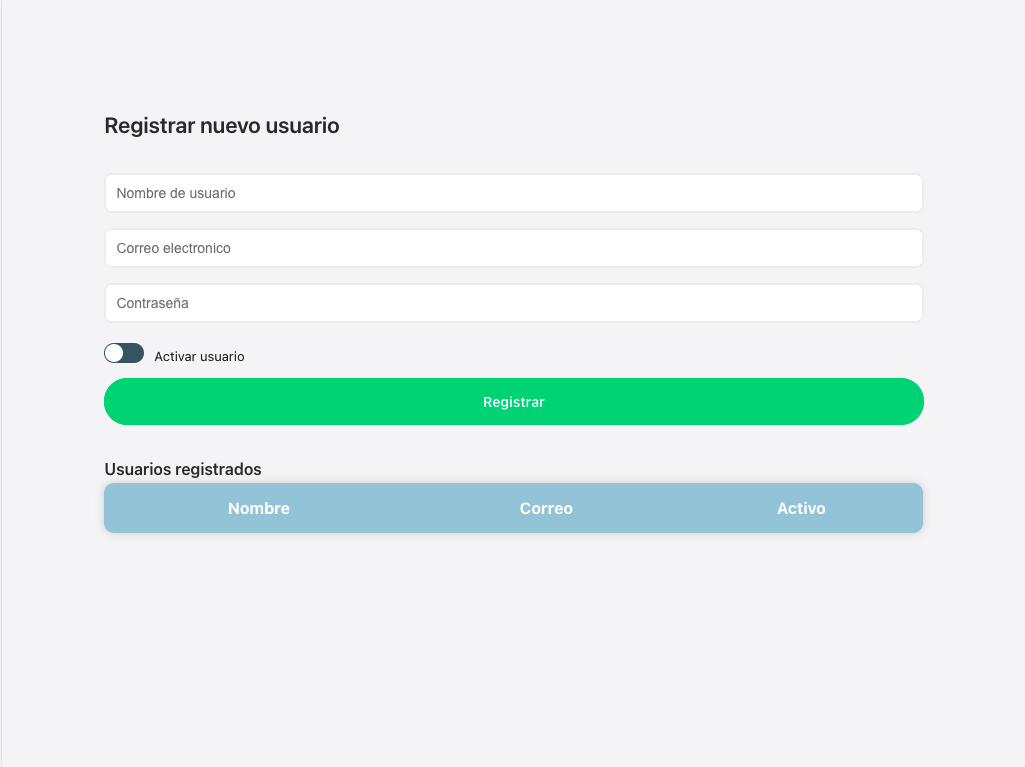
\includegraphics[width=1\textwidth]{./Imagenes/9.10}
   \centering 
    \caption[Resultado final]{Resultado final}
    \end{figure}
\newline
También se tiene el resultado después de agregar algunos usuarios.
\newline
\begin{figure}[H]
    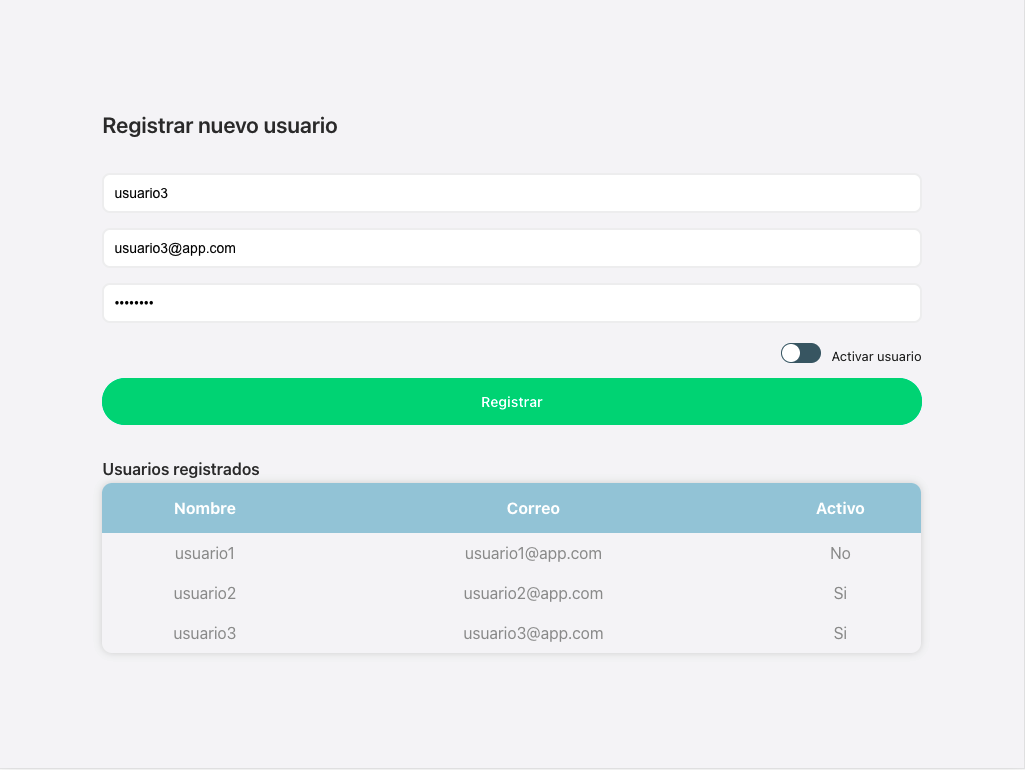
\includegraphics[width=1\textwidth]{./Imagenes/9.11}
   \centering 
    \caption[Resultado final al agregar usuarios]{Resultado final al agregar usuarios}
    \end{figure}
\newline
Los datos que se agregaron en la tabla, solo están almacenados en la memoria volátil del navegador, ya que esta biblioteca no cubre el hacer la petición HTTP. Pero la biblioteca es capaz de usarse con cualquier otra biblioteca que se encargue de hacer las peticiones por ejemplo AXIOS \cite{axios} (Cruz, R. 2019, November 1).

En seguida se muestra otro ejemplo que figura un restaurante en el cual se muestran los platillos que se venden, con la posibilidad de filtrarlos si son bebidas o tragos.

En el estado de React se tiene solamente un dato, este es el modo por el cual se están filtrando los datos.
\newline
\begin{figure}[H]
    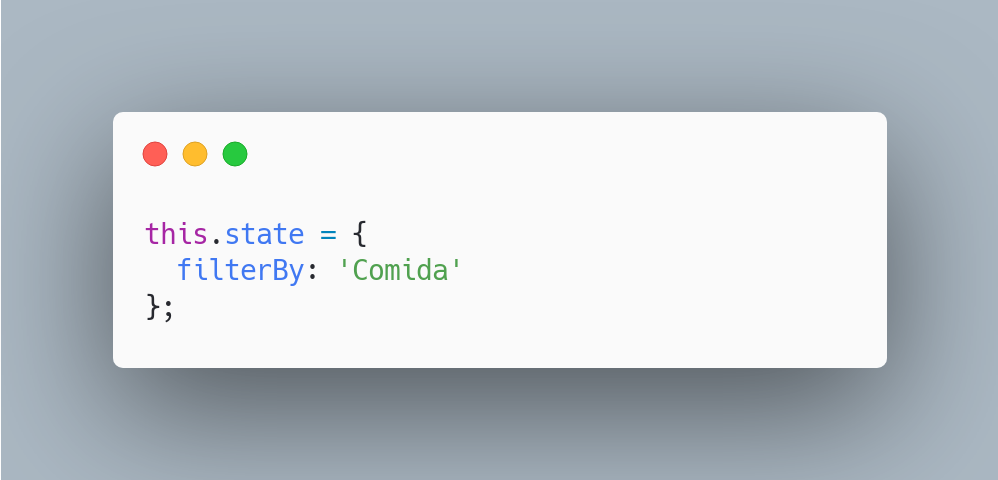
\includegraphics[width=0.7\textwidth]{./Imagenes/9.11-2}
   \centering 
    \caption[Filtro en el estado de React]{Filtro en el estado de React}
    \end{figure}
\newline

El código para maquetar los platillos es el siguiente el cual puede ser usado por ejemplo para la Web de un restaurante la cual recibe los datos de algún otro servicio Web.
El código de la siguiente Web cuenta con elemento DropDown que permite filtrar para mostrar comida o tragos las opciones posibles para mostrar son enviadas por el parámetro options, stateName es el nombre de llave que almacena la opción por la que se filtra, y también se tiene optionSelected que es en si el filtro.

Después se tiene un ciclo en el que se agrega cada uno de los platillos, el componente Card recibe el título de la tarjeta, la imagen y el contenido.
\newline
\begin{figure}[H]
    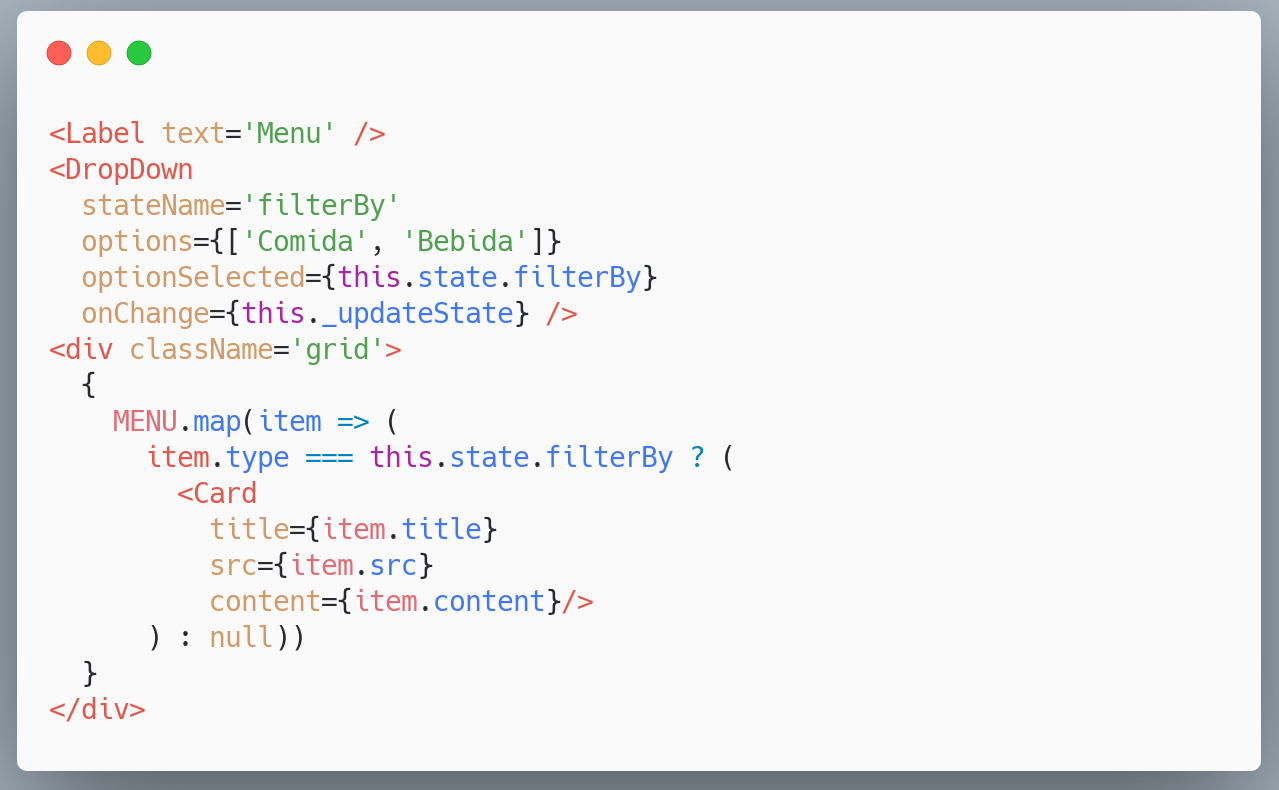
\includegraphics[width=1\textwidth]{./Imagenes/9.12.png}
   \centering 
    \caption[Código para mostrar los platillos]{Código para mostrar los platillos}
    \end{figure}
\newline

En las siguientes imágenes se muestra el resultado del código.
\newline
\begin{figure}[H]
    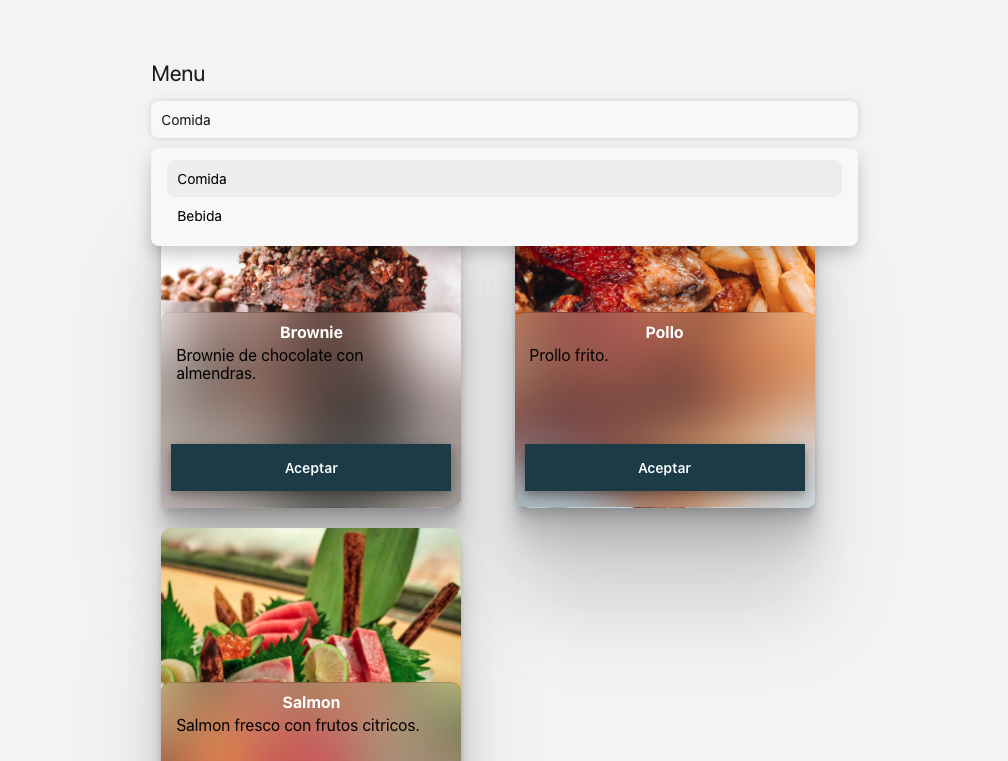
\includegraphics[width=1\textwidth]{./Imagenes/9.13.png}
   \centering 
    \caption[Filtrar por comida]{Filtrar por comida}
    \end{figure}
\newline

\newline
\begin{figure}[H]
    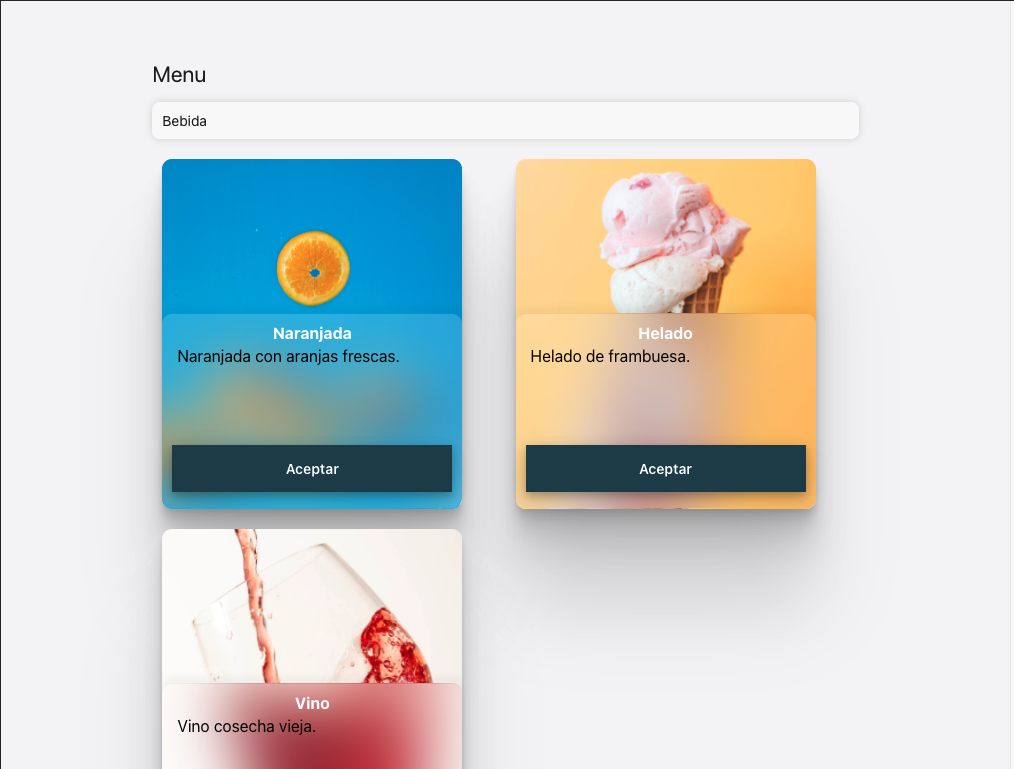
\includegraphics[width=1\textwidth]{./Imagenes/9.14.png}
   \centering 
    \caption[Filtrar por bebida]{Filtrar por bebida}
    \end{figure}
\newline

También se cuenta con el elemento Modal que puede ser usado como confirmación cuando el comprador presiona el botón para comprar un platillo.
\newline
\begin{figure}[H]
    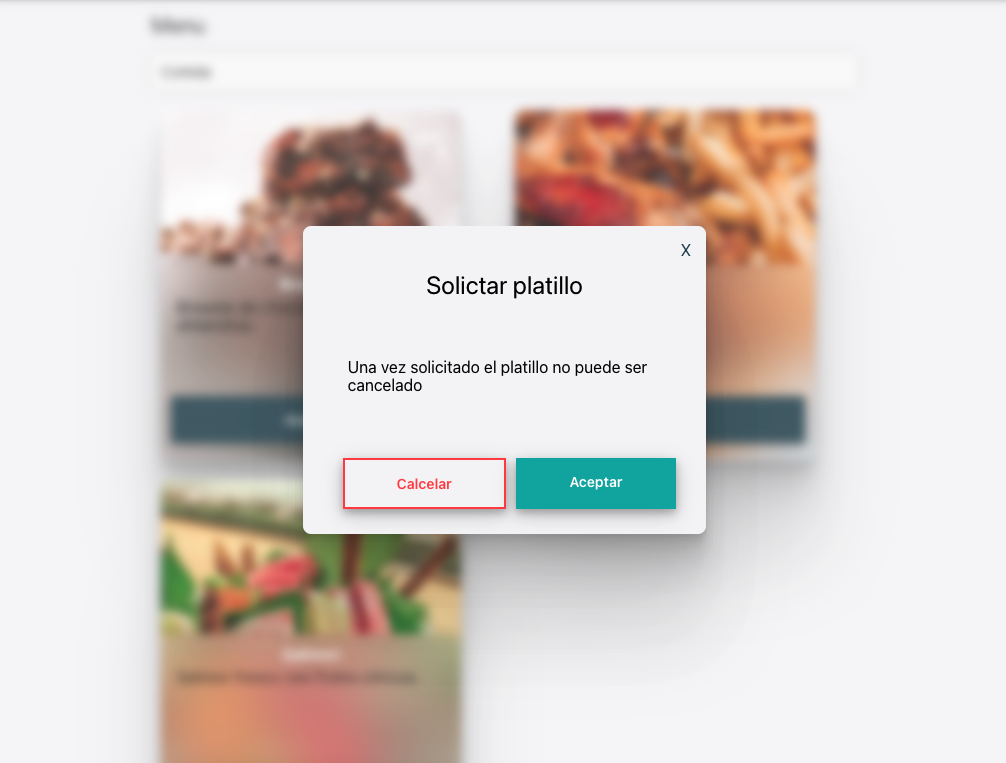
\includegraphics[width=1\textwidth]{./Imagenes/9.15.png}
   \centering 
    \caption[Confirmación de pedido]{Confirmación de pedido}
    \end{figure}
\newline

Los datos para mostrar los diferentes platillos no son obtenidos desde una petición HTTP, estos son tomados desde un array que existe sólo mientras la aplicación está en ejecución, ya que la biblioteca funciona para el Front-end.  Se puede implementar cualquier tecnología para hacer peticiones y obtener datos.

\section{Comparación contra Material Design}

  \begin{itemize}
   \item \textbf{ Número de componentes:} La biblioteca Material Design ya tiene algún tiempo de desarrollo, razón por la cual ya cuenta con gran cantidad de componentes, puedes encontrar múltiples opciones para cualquier necesidad, en contraste la biblioteca que aquí se desarrolla tiene un número limitado de componentes, que se considera que son los básicos usados en cualquier componente.
   \item \textbf{ Facilidad de uso:} Como ya se mencionó, Material Design tiene variedad de componentes, pero también gran cantidad de opciones que se pueden modificar, lo cual presenta una desventaja ya que si un nuevo desarrollador comienza a utilizar Material Design tendrá una mayor curva de aprendizaje, con respecto a nuestra biblioteca.
   \item \textbf{ Documentación:} Por el tiempo que tiene Material Design, ya tiene una gran cantidad de personas que lo saben usar, y foros en en los que se habla sobre funcionamiento y dan consejos para un mejor uso.
   \item \textbf{ Híbrido:} Material Design está diseñado para ser una biblioteca Front-end, pero nuestra biblioteca va más allá, la biblioteca que aquí se desarrolla para trabajar cien por ciento de la mano con el estado de react. 
   \item \textbf{ Peso:} Para comprobar el peso que requiere la biblioteca, se crean dos proyectos básicos de React \cite{CRA}  llamados pryectoCrown y proyectoMaterial, para el primero se instalará la biblioteca aquí desarrollada y en el segundo se instalará Material Design.
Al momento de crear las carpetas cada una tiene un peso de 241 MB, esto por el peso de la carpeta conocida node modules que guarda todas las dependencias.
Después se instaló cada una de las bibliotecas, el los proyectos. Una vez las bibliotecas instaladas el peso final de cada archivo fue el siguiente.

 \begin{itemize}
  \item \textbf{pryectoCrown:}  249 MB
   \item \textbf{proyectoMaterial:}   267 MB
 \end{itemize}
 Lo que nos da una diferencia de 18 MB de nuestra biblioteca con respecto a Material Design.
  \end{itemize}



